\Section{Analysis- Strategy and Setup}
\label{ch:analysis_strategy}

In this chapter, an overview of the analysis- strategy and setup will be given with a special focus on the physical observable used as the condition for the cINN inference.

\Subsection{Analysis Strategy}

The analysis has been performed on Monte Carlo (MC) data exclusively. The phase space in consideration has been selected to contain the highest signal yield. Hence the $gg \rightarrow WH \rightarrow b\bar{b} l\nu_l$ and $gg \rightarrow ZH \rightarrow b\bar{b}l\bar{l}$ final states have been considered. The Feynman diagram of these processes are shown in fig. \ref{fig:VH_finalstates}. Note that due to their weakly-interacting nature, neutrinos cannot be reconstructed in the detector. For this reason, former will be referred to as semi-leptonic and the latter as di-leptonic final state with lepton meaning electrons and/or muons exclusively.

\begin{table}[h!]
	\centering
%	\includegraphics[width=\linewidth]{imagefile}
	\begin{tabular}{c|c}
		Gluon Fusion & Quark Initiated \\
		\hline
		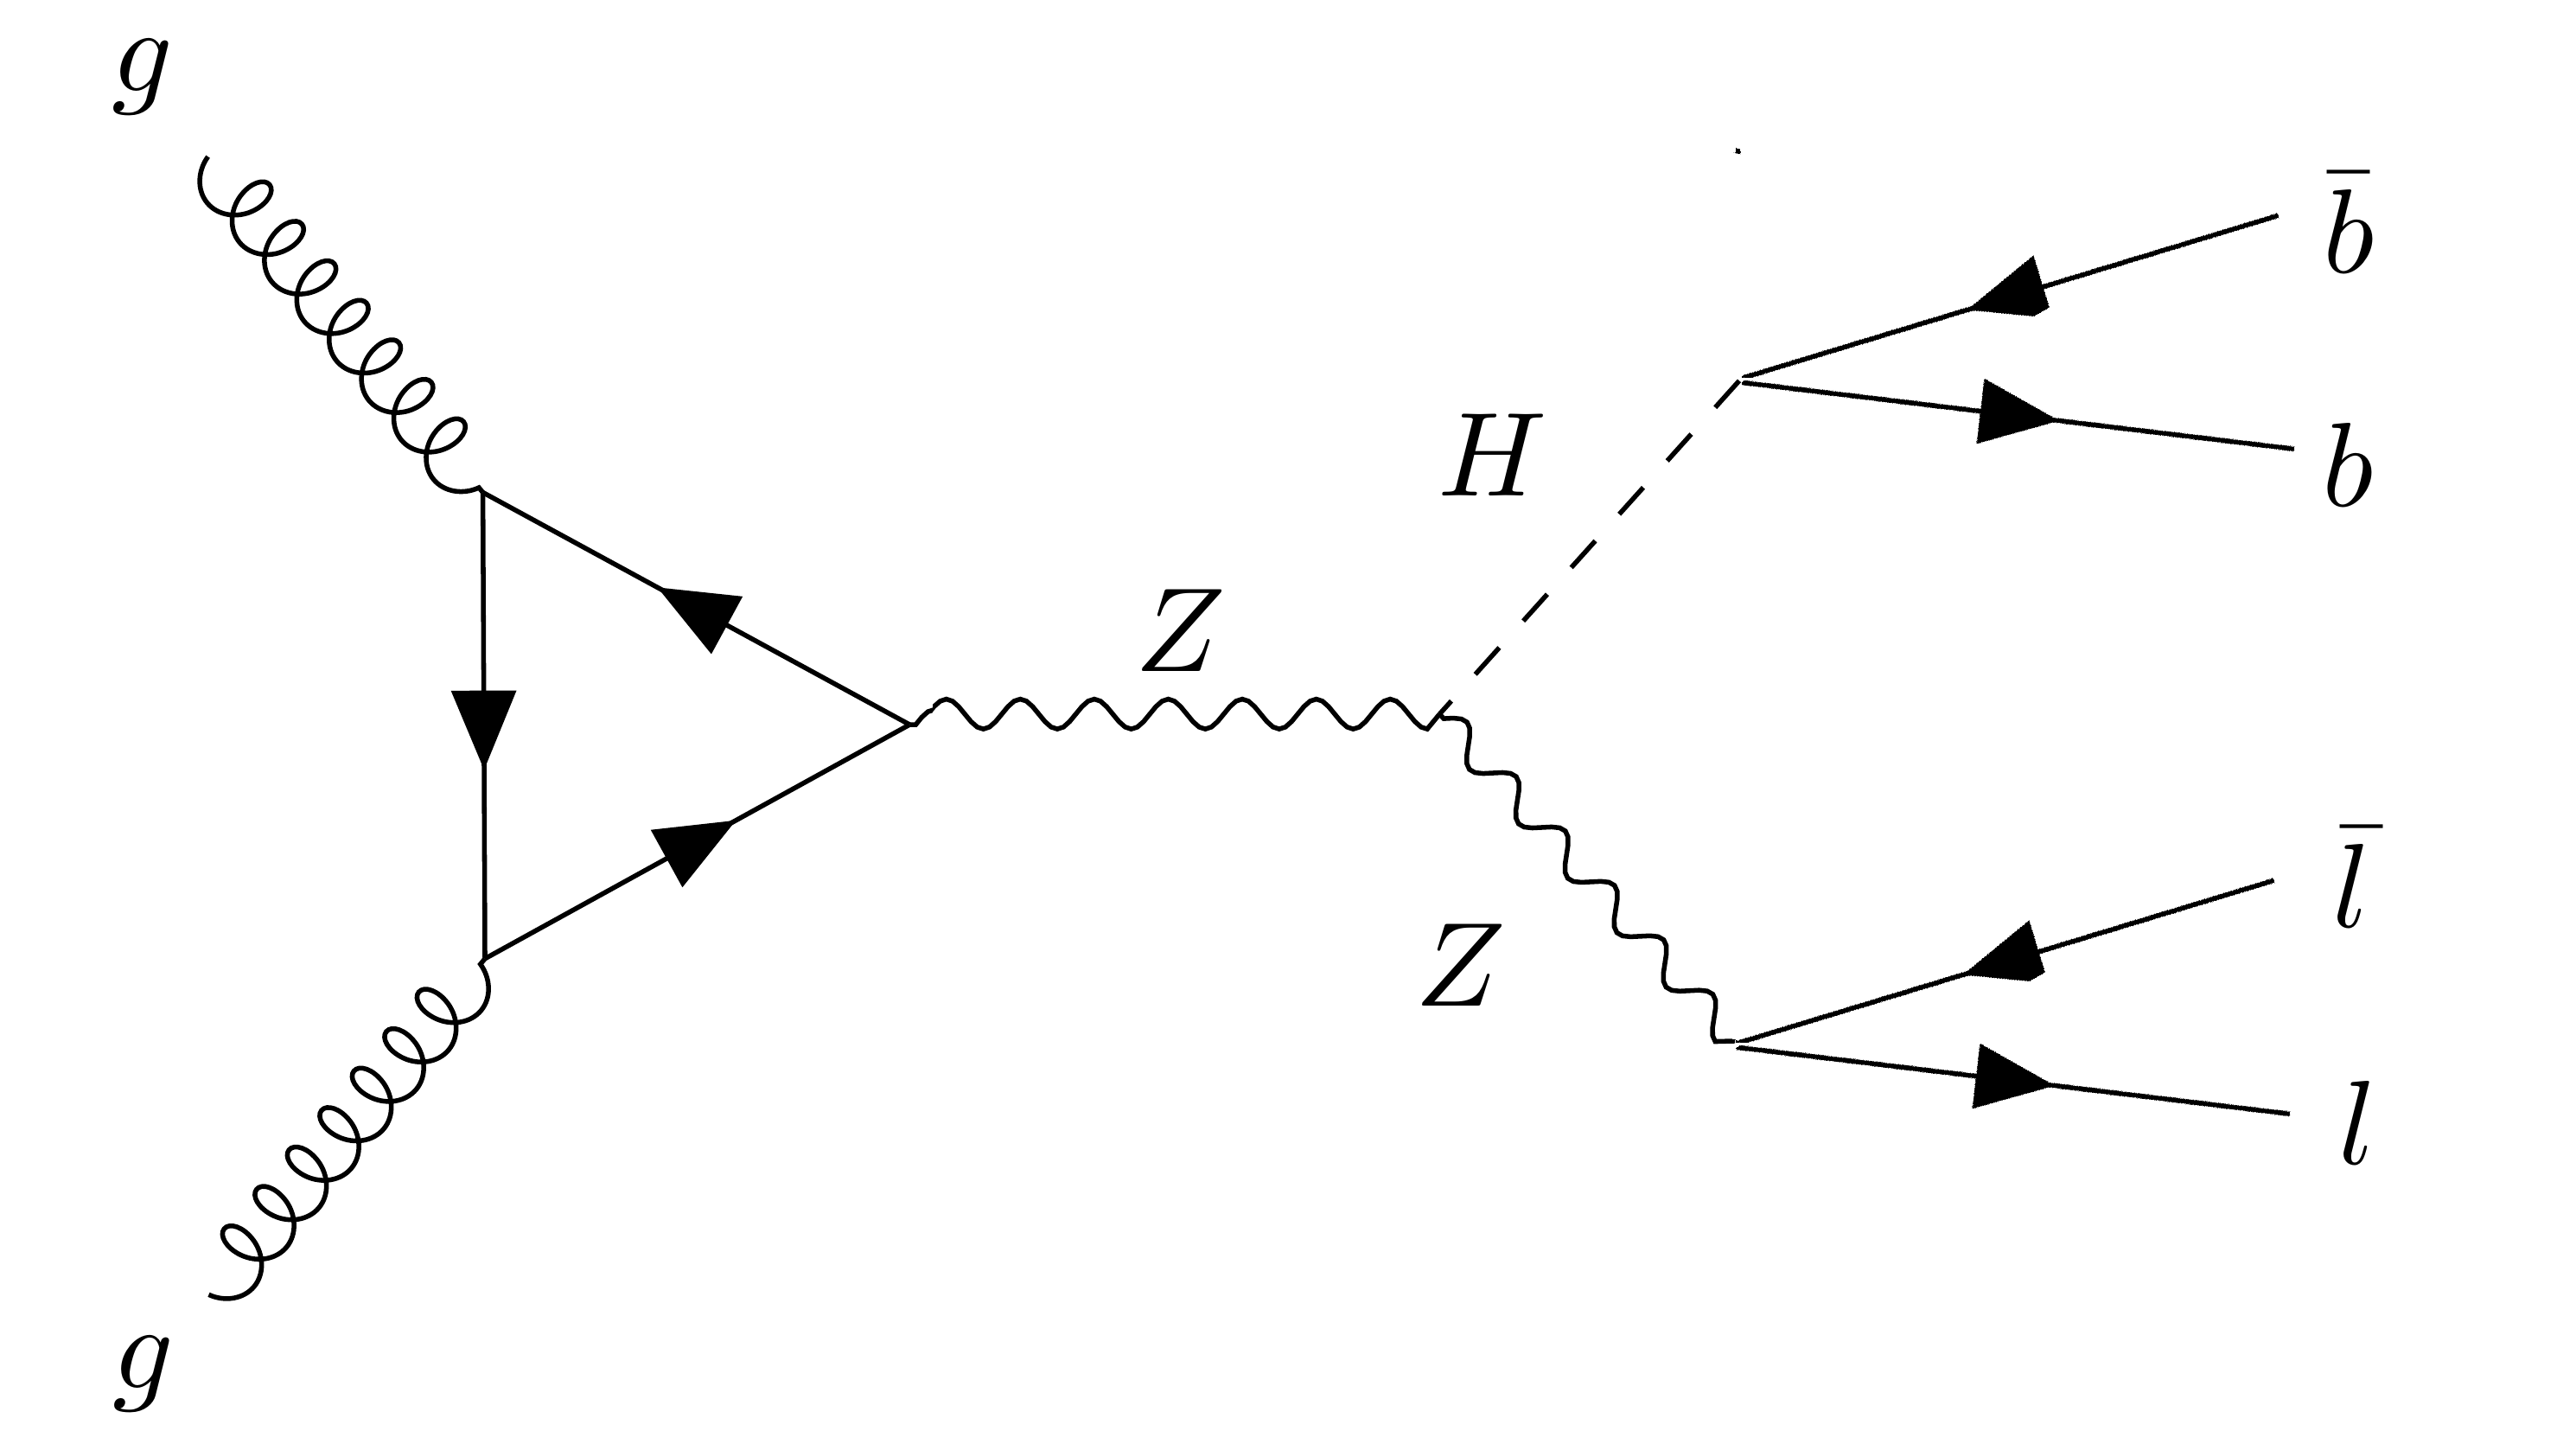
\includegraphics[width=0.4\linewidth]{figures/analysis/ggZH_triangle_bbll}&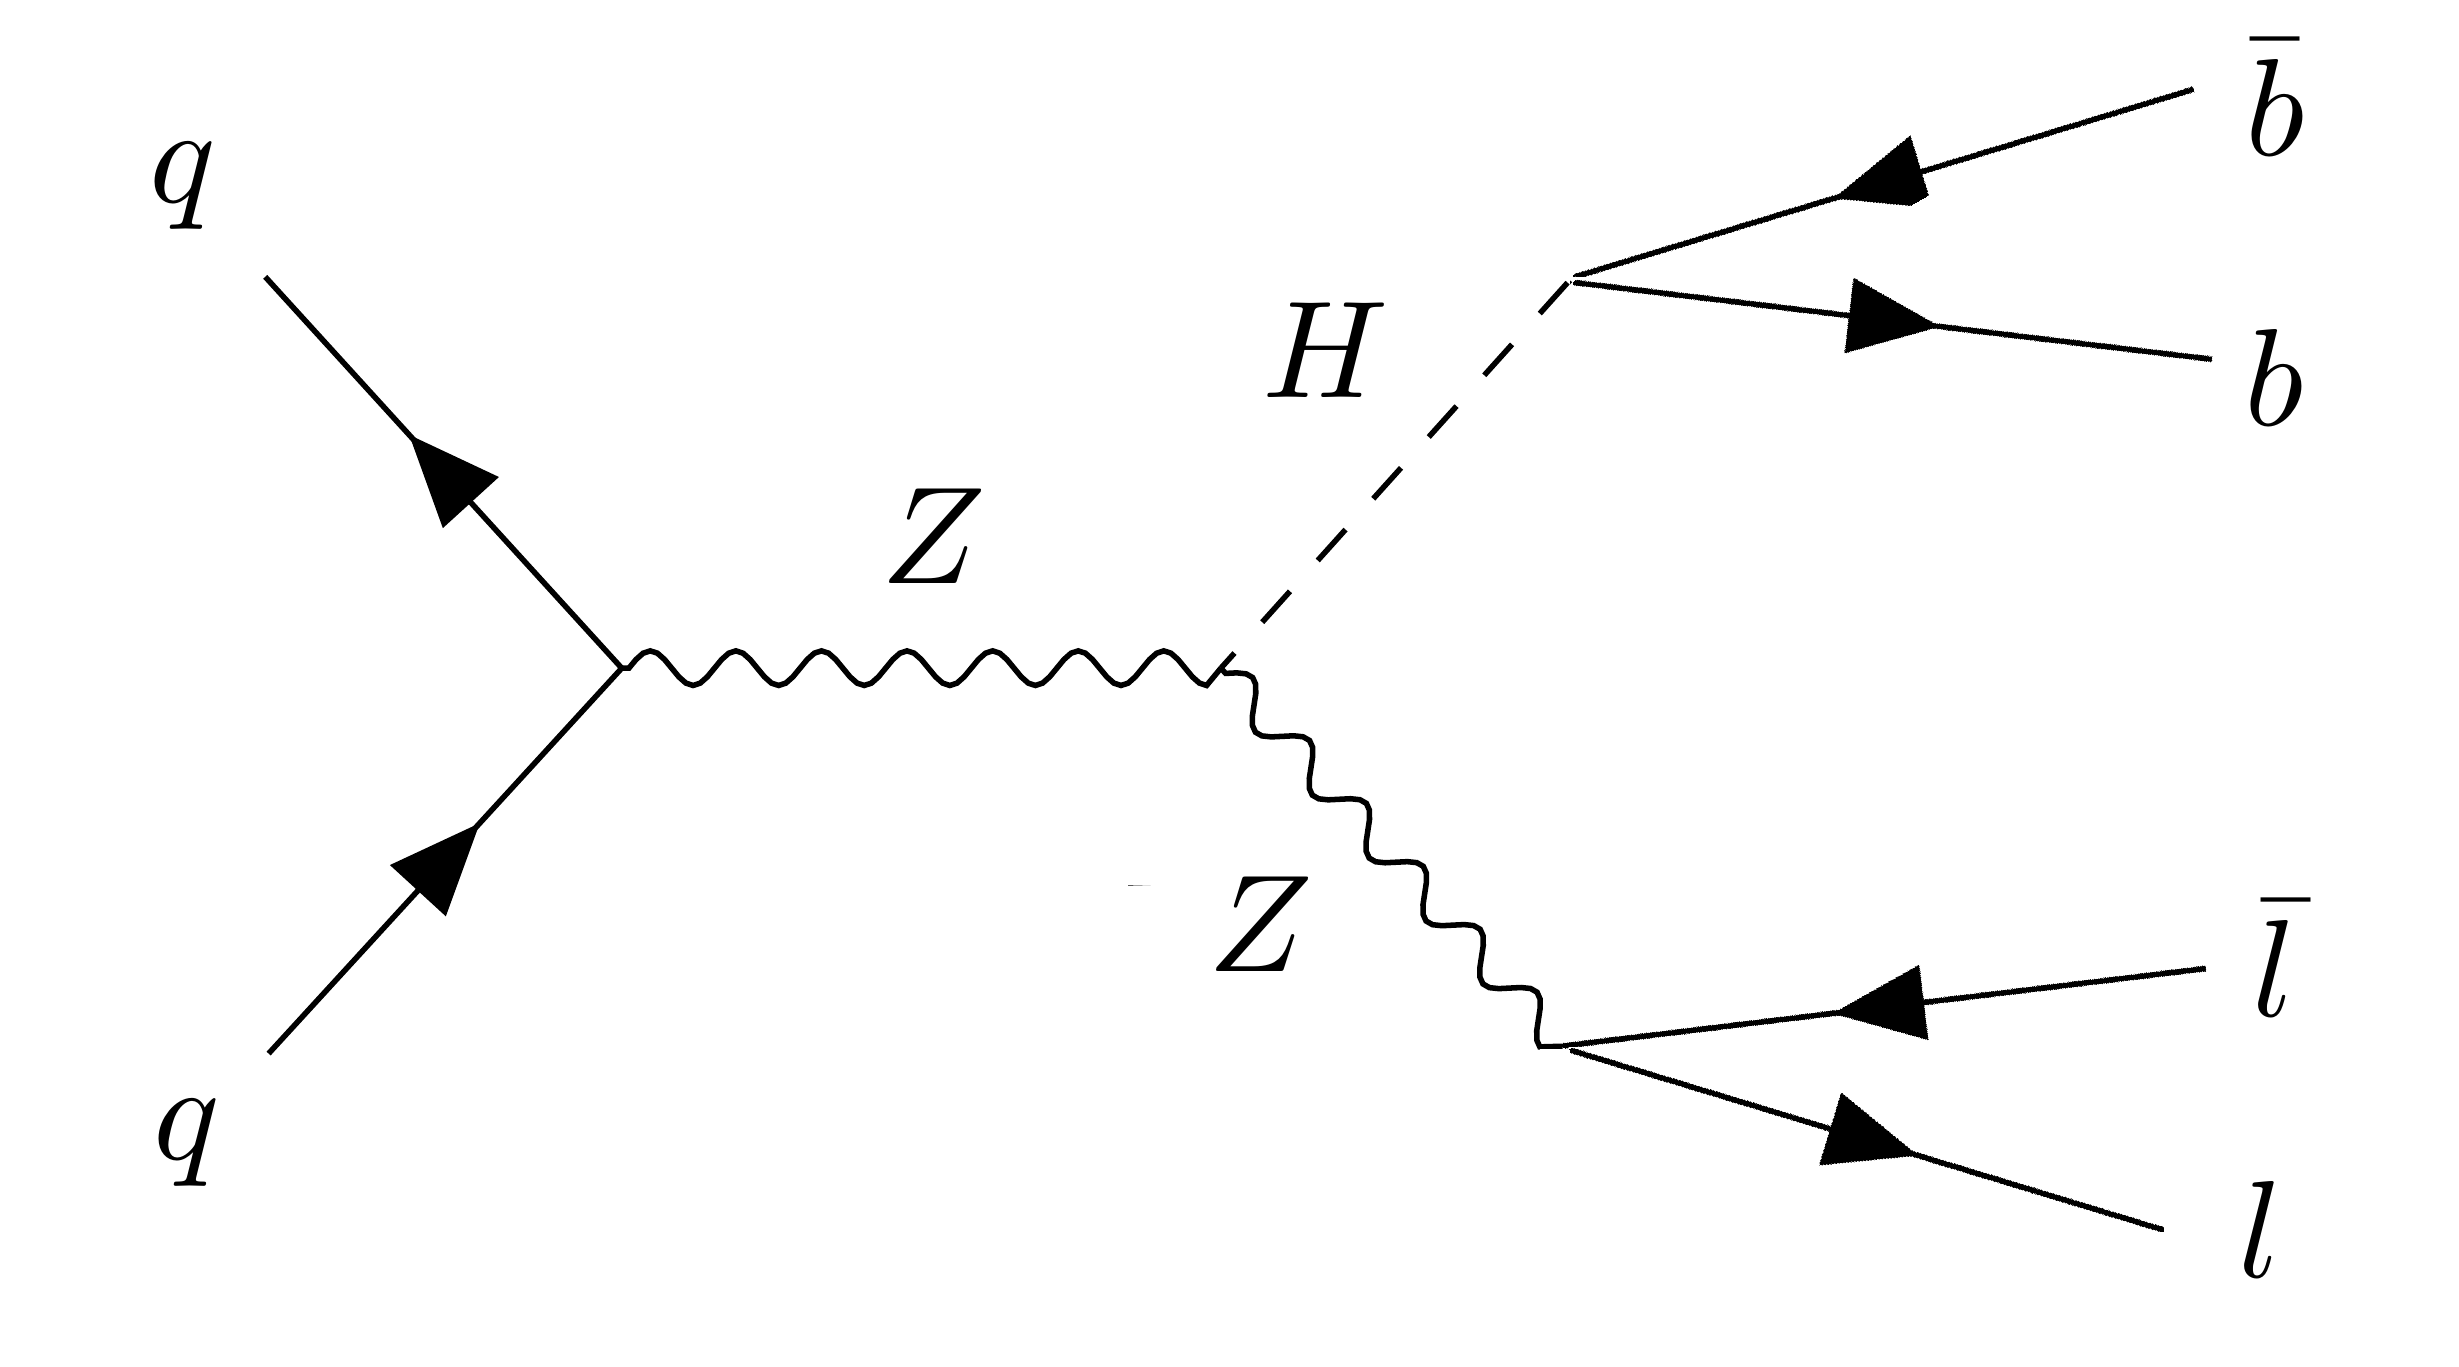
\includegraphics[width=0.4\linewidth]{figures/analysis/ZH_DY_bbll}  \\
		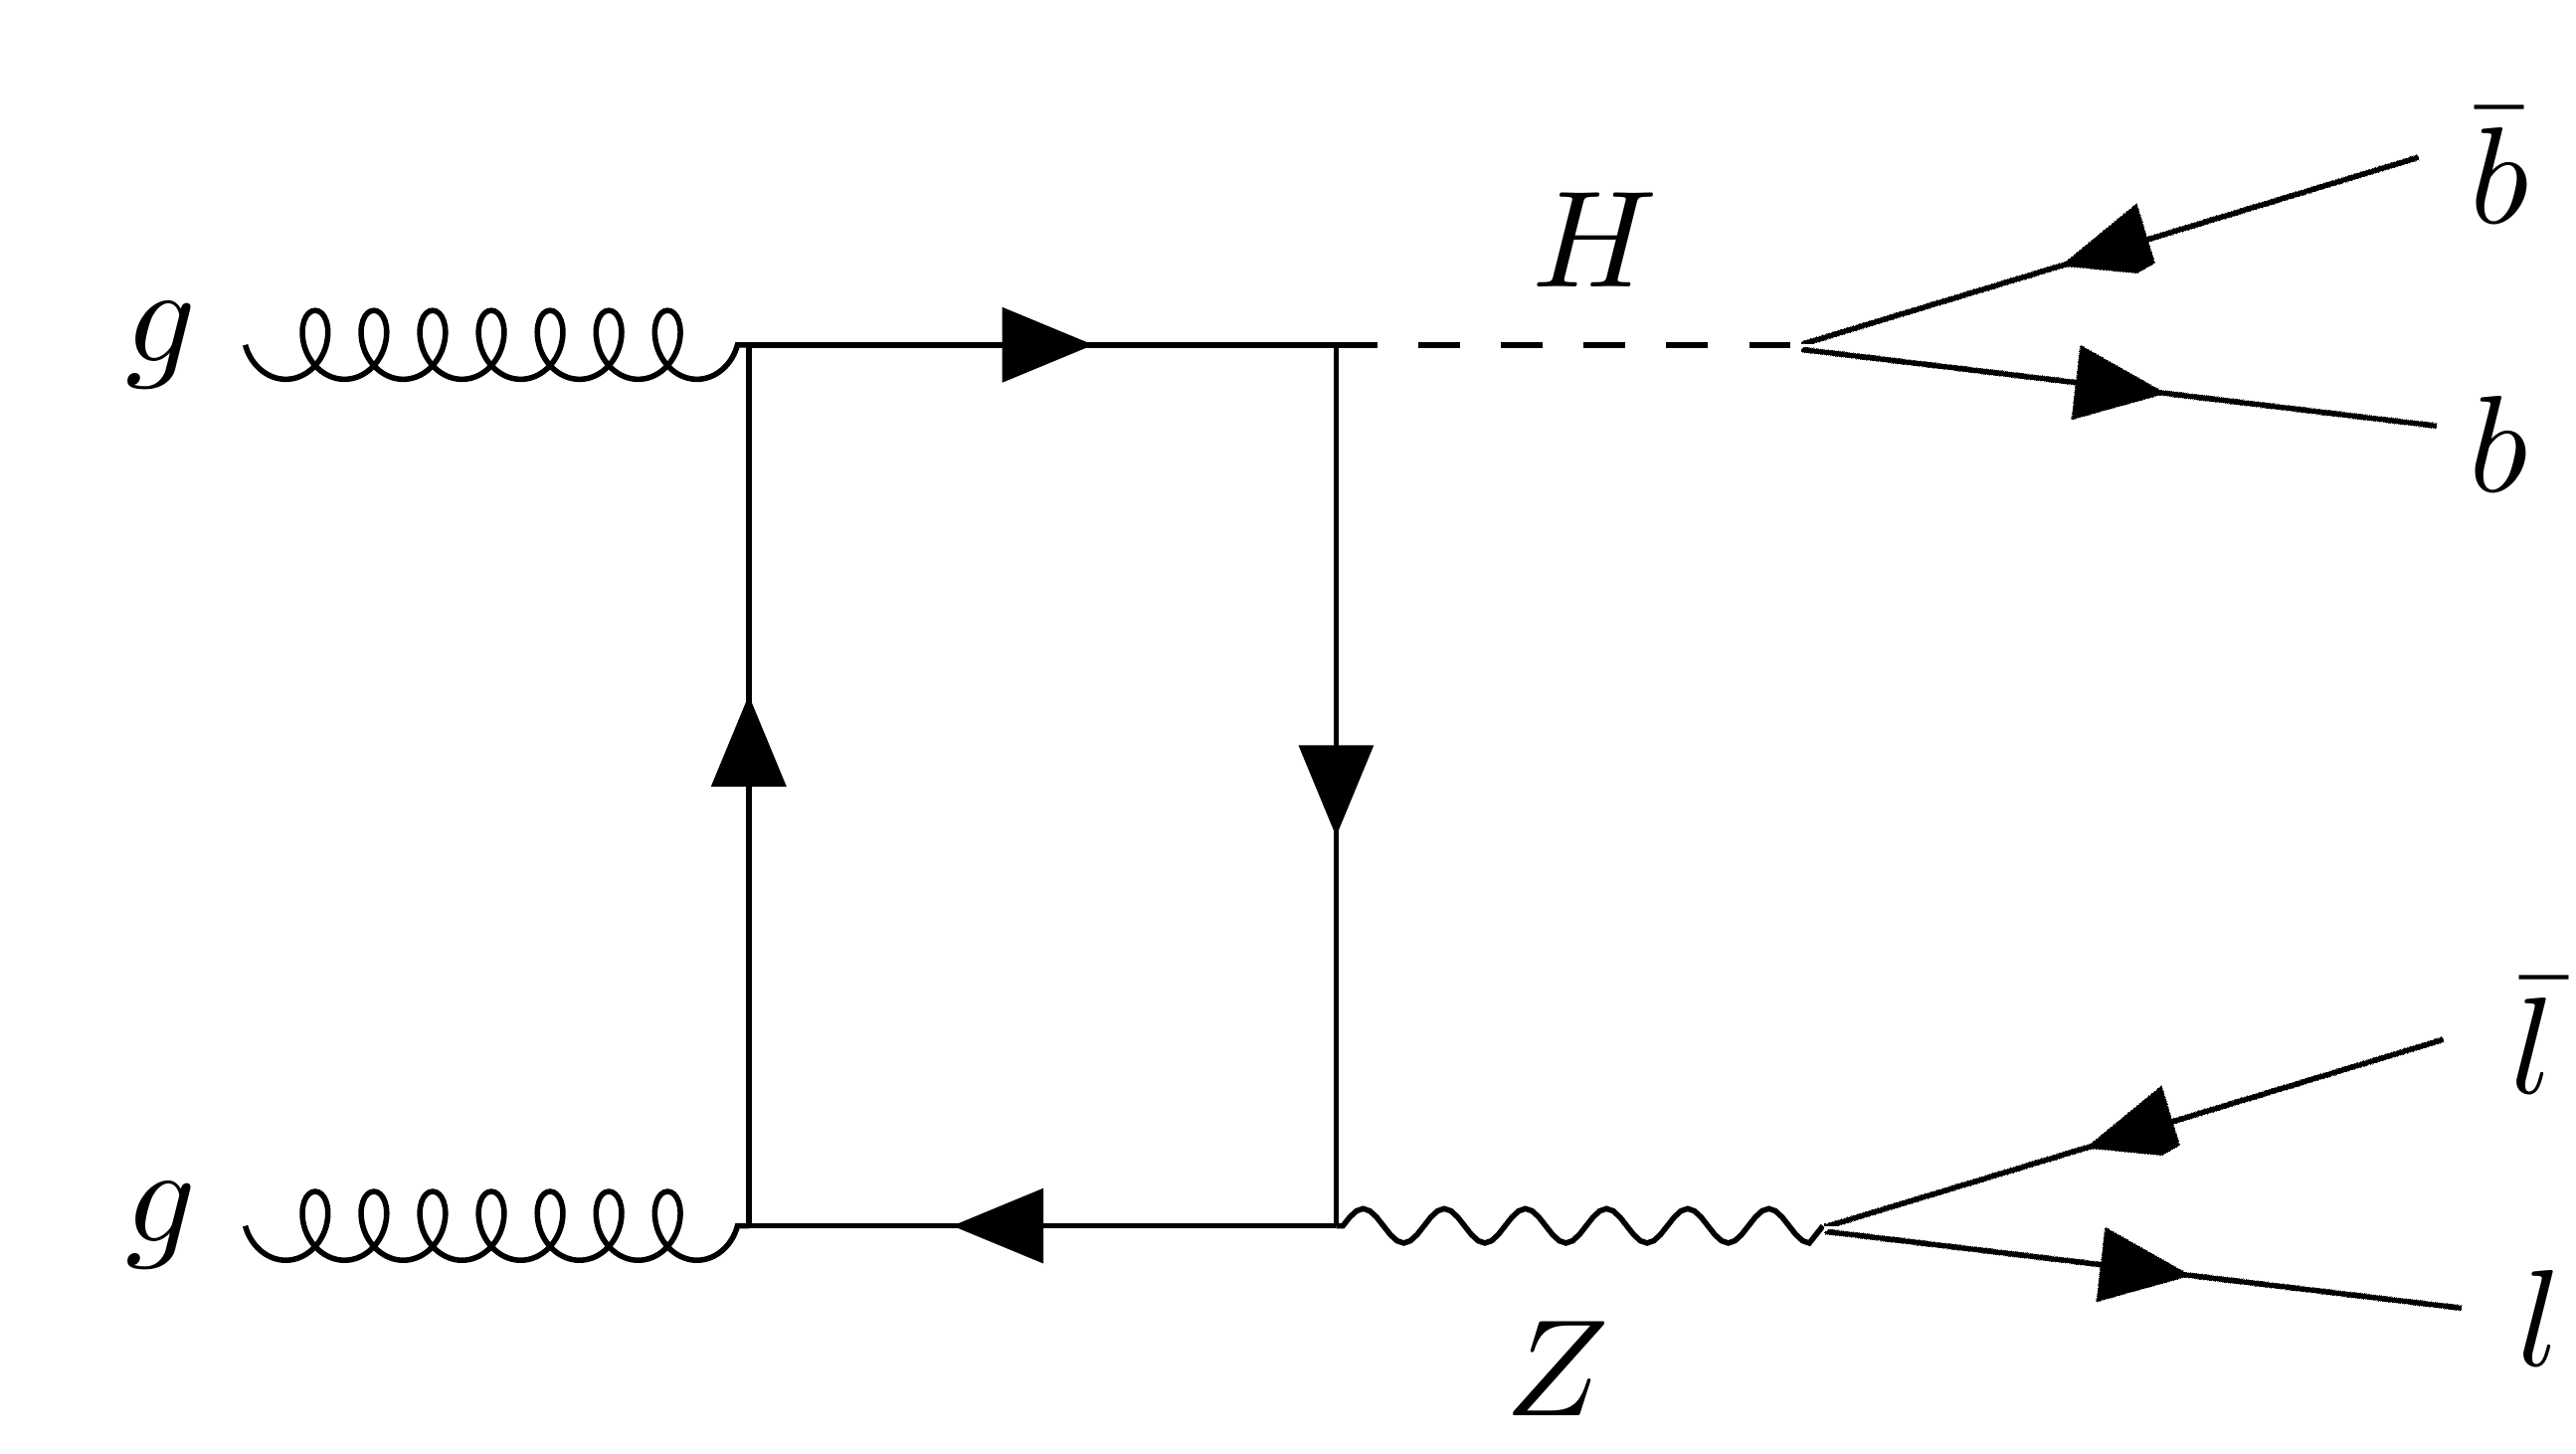
\includegraphics[width=0.4\linewidth]{figures/analysis/ggZH_box_bbll}& 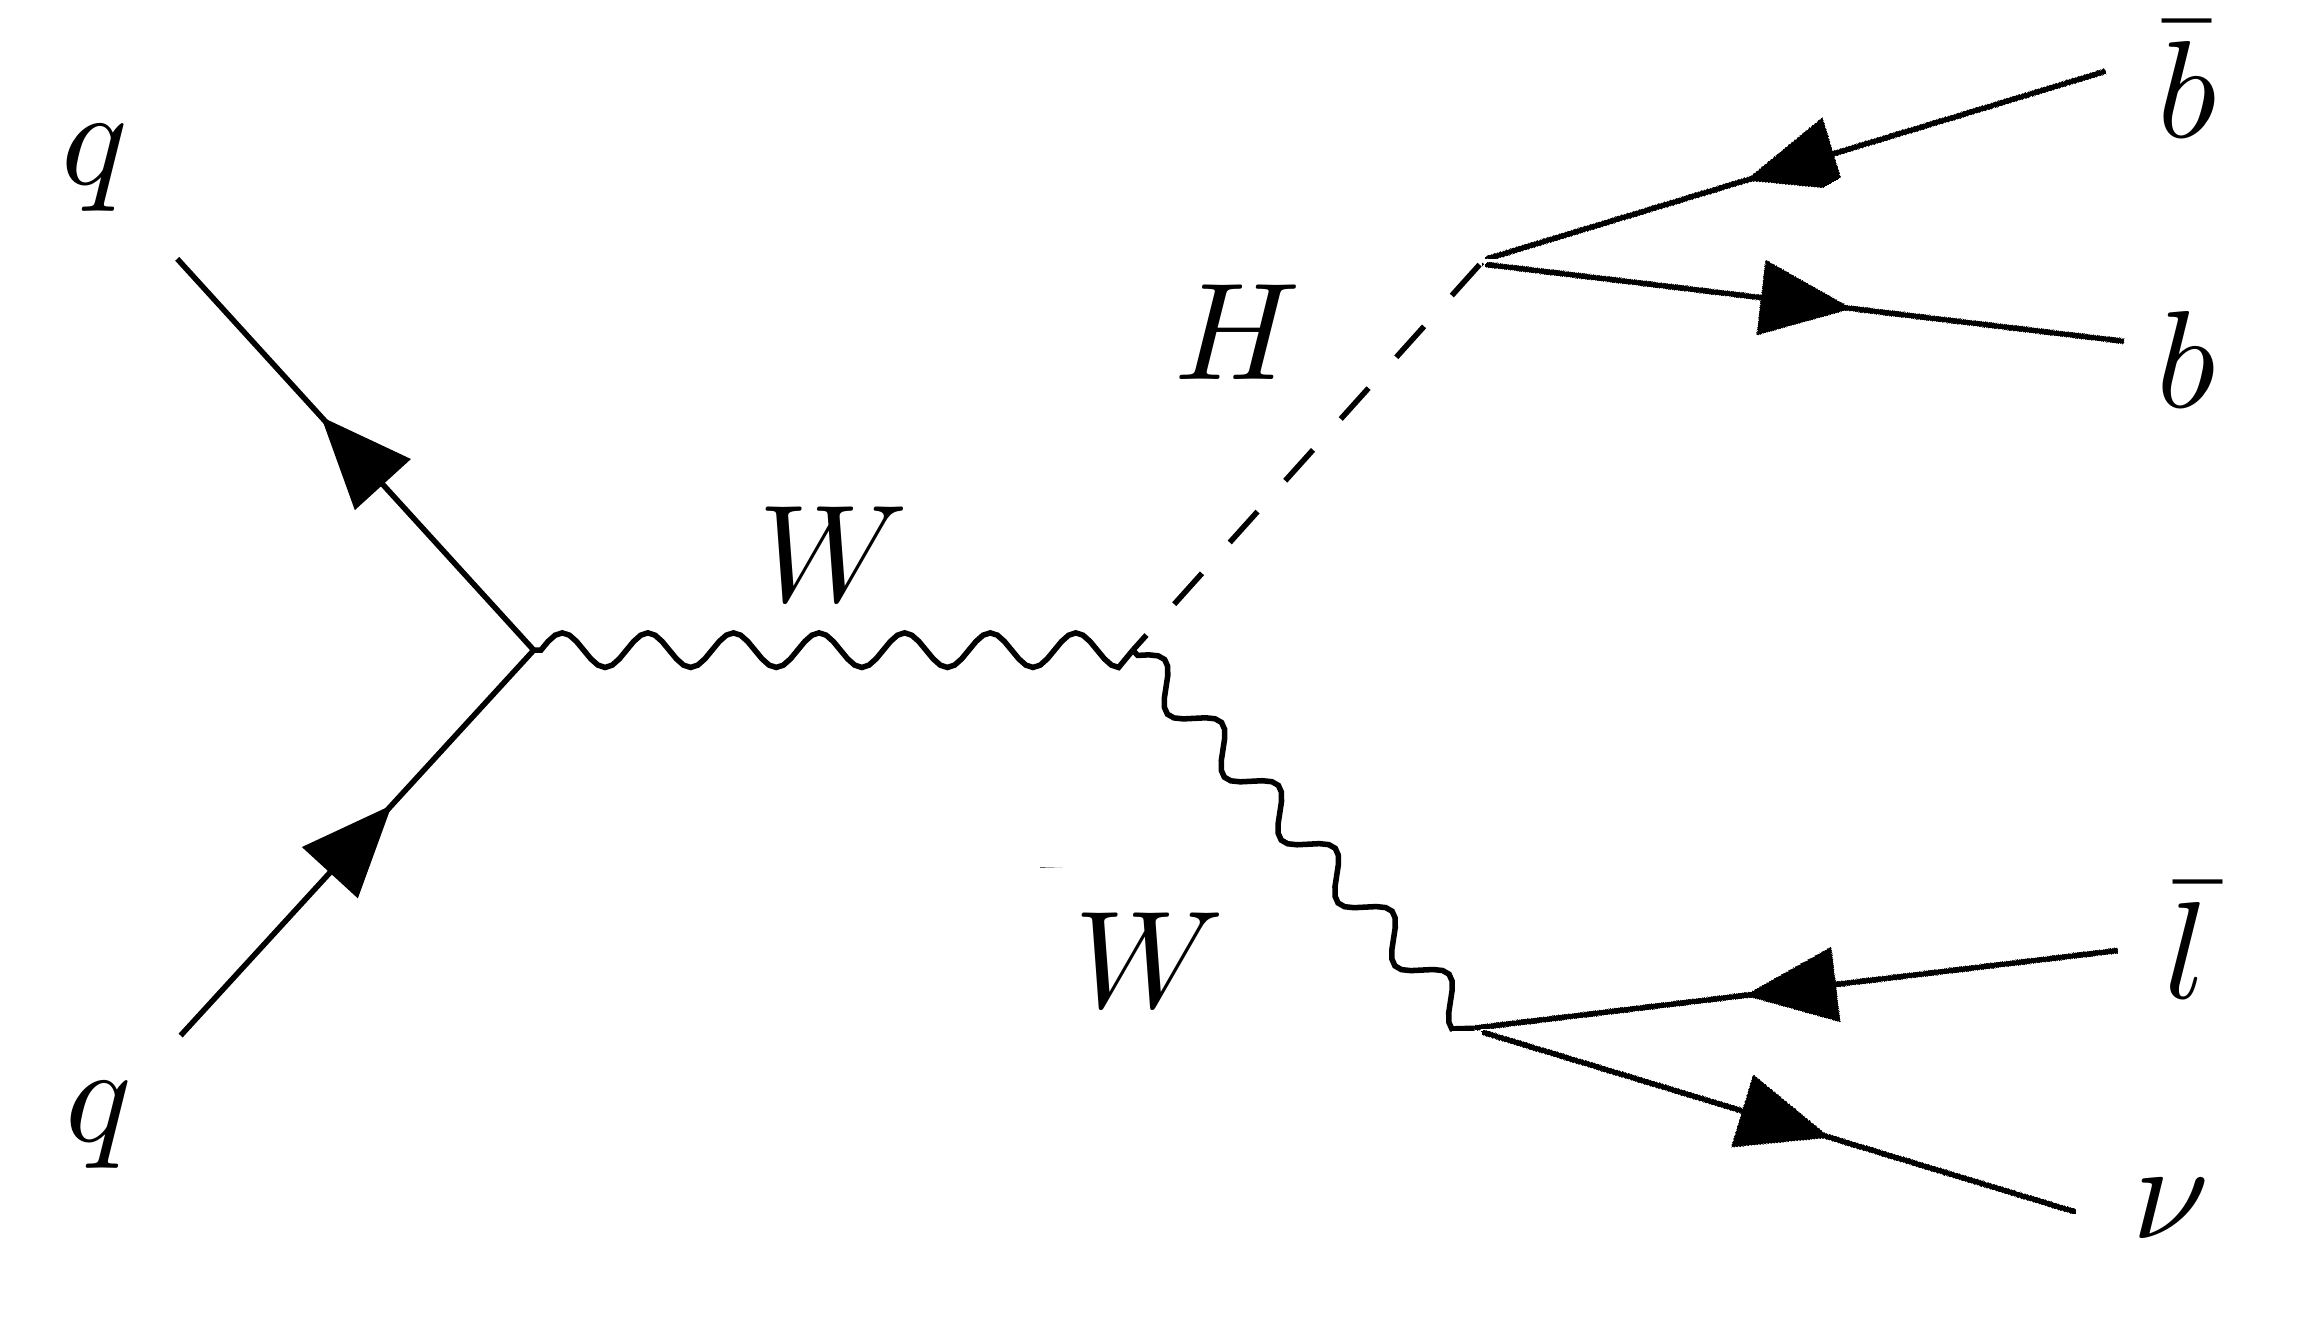
\includegraphics[width=0.4\linewidth]{figures/analysis/HWbbl} \\
	\end{tabular}
	\caption{The analysed final states of the $VH$ processes.}
	\label{fig:VH_finalstates}
\end{table}

The events are categorized through a triggering system and are assigned to one of four channels. The list of the triggers for the di- and semileptonic channels are listed in tab. \ref{tab:triggers}.

\begin{table}[h!]
	\centering
	\begin{tabular}{cc}
		Channel & Trigger Name \\
		\hline 
		\multirow{2}{*}{$ee$} & \texttt{Ele23\_Ele12\_CaloIdL\_TrackIdL\_IsoVL} \\
		& \texttt{Ele23\_Ele12\_CaloIdL\_TrackIdL\_IsoVL\_DZ} \\
		\hline 
		\multirow{2}{*}{$e$} & \texttt{Ele32\_WPTight\_Gsf} \\
		& \texttt{Ele32\_WPTight\_Gsf\_L1DoubleEG} \\
		\hline 
		\multirow{2}{*}{$\mu\mu$} & \texttt{Mu17\_TrkIsoVVL\_Mu8\_TrkIsoVVL\_DZ} \\
		& \texttt{Mu17\_TrkIsoVVL\_Mu8\_TrkIsoVVL\_DZ\_Mass3p8} \\
		\hline 
		\multirow{2}{*}{$\mu$} & \texttt{IsoMu24\_eta2p1} \\
		& \texttt{IsoMu27} \\
		\hline \\
	\end{tabular}
	\caption{The lepton triggers used in the analysis.}
	\label{tab:triggers}
\end{table}

The naming in tab. \ref{tab:triggers} indicates the phase space which the triggers cut off. In the di-leptonic channels the lepton with the higher energy (the leading lepton) is required to have $p_T > \SI{23}{\giga\electronvolt}$ and $p_T > \SI{17}{\giga\electronvolt}$ for $ee$ and $\mu\mu$, respectively; the sub-leading (the "other") lepton is then required to have $p_T>\SI{12}{\giga\electronvolt}$ and $\SI{8}{\giga\electronvolt}$ for $ee$ and $\mu\mu$, respectively. In the semi-leptonic categories, only electrons with $p_T>\SI{32}{\giga\electronvolt}$ and isolated muons with $\SI{24}{\giga\electronvolt}$ and $|\eta|<2$ and isolated muons with $p_T>\SI{27}{\giga\electronvolt}$ are kept.

In addition to these selection criteria, both muon tracks have to be isolated in the $\mu\mu$ channel. For the $e$ channel, the tight working point has been selected as trigger efficiency.

The datasets used for the analysis have been simulated with \texttt{PYTHIA} \cite{Sj_strand_2008} and \texttt{HERWIG++} \cite{herwig}. These simulated events not only contain matrix element calculation samples, but also the CMS detectors simulations using \texttt{GEANT4} in order to represent the final expected distributions accurately \cite{geant1, geant2, geant3}. The list of the signal sample datasets is shown in tab. \ref{tab:signal_datasets}. These processes are \texttt{ggZH} (for the box diagram process), \texttt{ZH\_DY} (for the Drell-Yan-like $ZH$ production process) and \texttt{WH} (for the $WH$ Higgsstrahlung process).

\begin{table}[h!]
	\centering
	\begin{tabular}{lS[table-format=8.0]S[table-format=1.6]}
%		\toprule
		Dataset name&{N}&$\sigma/$\si{\pico\barn} \\
		\midrule
		\verb|ZH_HToBB_ZToLL_M125_13TeV_powheg_pythia8|&9530684 &0.04471\\
		\verb|ggZH_HToBB_ZToLL_M125_13TeV_powheg_herwigpp|& 199131&0.00722\\
		\midrule
		\verb|WminusH_HToBB_WToLNu_M125_13TeV_powheg_pythia8|&2382500&0.1012\\
		\verb|WplusH_HToBB_WToLNu_M125_13TeV_powheg_pythia8|&2481200&0.1595\\
%		\bottomrule
	\end{tabular}
	\caption{Simulated signal samples for the quark initiated ZH- and WH- and gluon fusion induced ZH process for 2017, with the cross section $\sigma$ of each process and the number of generated events $N$.}
%	\caption{\textcolor{red}{The signal datasets}}
	\label{tab:signal_datasets}
\end{table}

Regarding (ir)reducible background, one distinguishes between the following processes:

\begin{itemize}
	\item[] \texttt{dy}: Drell-Yan-like vector boson production with hadronic initial state radiation. This process has high cross section and yields the same final state (for radiated bottom jets) as the signal. In addition, it has the same lepton signature too. The process is shown in fig. \ref{fig:dy_background}.
	\begin{figure}[h!]
		\centering
		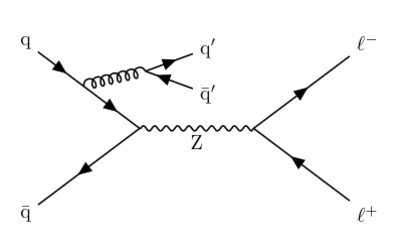
\includegraphics[width=0.4\textwidth]{figures/analysis/dy.pdf}
		\caption{The Feynman diagram for the dy background process.}
		\label{fig:dy_background}
	\end{figure}
	\item[] $\texttt{t}\bar{\texttt{t}}$: Production of top quark pairs $t\bar{t}$. These quarks decay via $t\rightarrow Wb$ and with the leptonic decay channel of the $W$, this has the same final state as the signal process. This has the second largest background contribution. The corresponding Feynman diagram is shown in fig. \ref{fig:tt_background}.
	\begin{figure}[h!]
		\centering
		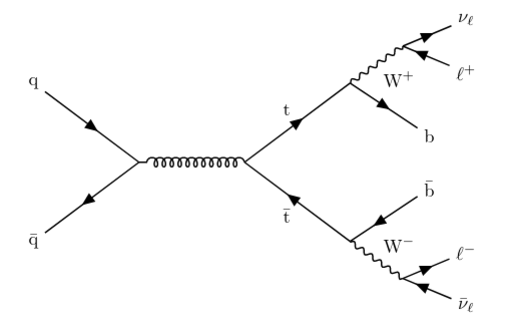
\includegraphics[width=0.5\textwidth]{figures/analysis/tt.pdf}
		\caption{The Feynman diagram for the tt background process.}
		\label{fig:tt_background}
	\end{figure}
	\item[] $\texttt{t}\bar{\texttt{t}}\texttt{V}$: Associated vector boson production in the initial or final states with a $t\bar{t}$ pair. For the top quarks decaying into bottom quarks and the leptonically decaying vector bosons, this yields a final state similar to the signal final state.
	\item[] $\texttt{st}$: Single top quark production. A hadronically decaying top with a QCD-induced bottom jet results in a semileptonic di-bottom state.
	\item[] \texttt{VV}, \texttt{VVV} and $\texttt{t}{\bar{\texttt{t}}}\texttt{VV}$: di- or triboson production with (or without) associated $t\bar{t}$ production. If any of these vector bosons decay hadronically while the other(s) decay leptonically, this results in a semi- or dileptonic di-bottom final state.
	\item[] $\texttt{t}\bar{\texttt{t}}\texttt{VH}$, \texttt{ggH} and \texttt{VBFH}: Higgs production channels.
	\item[] \texttt{wjets}: leptonically decaying jet-associated $W$ boson production.
	\item[] \texttt{QCD}: reducible QCD background.
	\item[] \texttt{rare}: rare processes (such as four top production) with individual low contribution each
\end{itemize}

The list of the background samples from the MC simulations are all listed in tab. \ref{tab:bkg_datasets}.

\begingroup
\footnotesize
\begin{longtable}[b]{llS[table-format=9.0]S[table-format=7.8]}
	\caption{List of simulated background samples for 2017 with the cross section $\sigma$ of each process and the number of generated events $N$, divided into process groups. The symbol \texttt{*} is a placeholder for \texttt{pythia8}, while \texttt{**} denotes \texttt{inclusiveDecays}. Long dataset names are split into multiple lines, denoted by an indentation. (NanoAODv7, 102X\_mc2017\_realistic\_v8-v1)}\\
	Process&Dataset name&{N}&$\sigma/$\si{\pico\barn} \\
	\midrule
	\endfirsthead
	\toprule
	Process&Dataset name&{N}&$\sigma/$\si{\pico\barn} \\
	\midrule
	\endhead
	\bottomrule
	\endfoot
	\bottomrule
	\endlastfoot
	
	\multirow{ 4}{*}{DY}&\verb|DYJetsToLL_M-10to50_TuneCP5_13TeV-madgraphMLM-*| & 79058069&18610.0\\
	&\verb|DYJetsToLL_0J_TuneCP5_13TeV-amcatnloFXFX-*| &88134822 &4843.6\\
	&\verb|DYJetsToLL_1J_TuneCP5_13TeV-amcatnloFXFX-*| & 95629091&897.8\\
	&\verb|DYJetsToLL_2J_TuneCP5_13TeV-amcatnloFXFX-*| & 54497574&335.8\\
	\midrule%t$\bar{\textrm{t}}$
	\multirow{ 3}{*}{t$\Bar{\textrm{t}}$}&\verb|TTTo2L2Nu_TuneCP5_PSweights_13TeV-powheg-*| & 68296294&88.4\\
	&\verb|TTToSemiLeptonic_TuneCP5_PSweights_13TeV-powheg-*| & 109795512&365.52\\
	&\verb|TTToHadronic_TuneCP5_PSweights_13TeV-powheg-*| &128829950&377.96\\
	\midrule
	\multirow{ 5}{*}{VV}&\verb|WWTo2L2Nu_NNPDF31_TuneCP5_PSweights_13TeV-powheg-*| & 2000000&12.2\\
	&\verb|WWTo2L2Nu_DoubleScattering_13TeV-*| & 968000&0.2232\\
	&\verb|ZZTo4L_13TeV_powheg_*| & 207798469&1.256\\
	&\verb|WZTo3LNu_TuneCP5_13TeV-amcatnloFXFX-*| & 10987679&4.43\\
	&\verb|ZGToLLG_01J_5f_TuneCP5_13TeV-amcatnloFXFX-*| & 30490034&55.59\\
	\midrule
	%&\verb|?WGToLNuG_TuneCP5_13TeV-madgraphMLM-*| &  6283083&464.800\\%aktuell auskommentiert
	%\midrule
	\multirow{ 7}{*}{ST}&\verb|ST_t-channel_top_4f_**_TuneCP5_13TeV-powhegV2-madspin-*| & 5982064&136.02\\
	&\verb|ST_t-channel_antitop_4f_**_TuneCP5_13TeV-powhegV2-madspin-*| & 3675910&80.95\\
	&\verb|ST_s-channel_4f_leptonDecays_TuneCP5_| & 9914948&3.364\\
	&\verb|     PSweights_13TeV-amcatnlo-*|\\
	&\verb|ST_tW_top_5f_**_TuneCP5_PSweights_13TeV-powheg-*| &7755138 &35.85\\
	&\verb|ST_tW_antitop_5f_**_TuneCP5_PSweights_13TeV-powheg-*| & 7745276&35.85\\
	&\verb|ST_tWll_5f_LO_TuneCP5_PSweights_13TeV-madgraph-*| & 986000&0.01096\\
	\midrule
	\multirow{ 5}{*}{VVV}&\verb|WWW_4F_TuneCP5_13TeV-amcatnlo-*| & 472300&0.2086\\
	&\verb|WWZ_4F_TuneCP5_13TeV-amcatnlo-*| & 500000&0.1676\\
	&\verb|WZZ_TuneCP5_13TeV-amcatnlo-*| & 500000&0.05701\\
	&\verb|ZZZ_TuneCP5_13TeV-amcatnlo-*| & 500000&0.01473\\
	&\verb|WZG_TuneCP5_13TeV-amcatnlo-*| & 1000000&0.04345\\
	\midrule
	\multirow{ 5}{*}{t$\Bar{\textrm{t}}$V}&\verb|TTZToLL_M-1to10_TuneCP5_13TeV-amcatnlo-*| &250000 &0.0822\\
	&\verb|TTZToLLNuNu_M-10_TuneCP5_PSweights_13TeV-amcatnlo-*| &11092000 &0.2814\\
	&\verb|TTZToQQ_TuneCP5_13TeV-amcatnlo-*| &9690000 &0.5868\\
	&\verb|TTWJetsToLNu_TuneCP5_PSweights_13TeV-amcatnloFXFX-madspin-*| & 9828579&0.196\\
	&\verb|TTWJetsToQQ_TuneCP5_13TeV-amcatnloFXFX-madspin-*| &811306 &0.4049\\
	\midrule
	\multirow{ 1}{*}{t$\Bar{\textrm{t}}$VV}&\verb|TTWW_TuneCP5_13TeV-madgraph-*| & 1162000&0.006981\\
	\midrule
	\multirow{ 2}{*}{t$\Bar{\textrm{t}}$VH}&\verb|TTWH_TuneCP5_13TeV-madgraph-*| & 200000&0.001582\\
	&\verb|TTZH_TuneCP5_13TeV-madgraph-*| & 200000&0.001535\\
	\midrule
	\multirow{ 9}{*}{ggH}&\verb|GluGluHToTauTau_M125_13TeV_powheg_*| &15072210 &3.0469\\
	&\verb|GluGluHToZZTo4L_M125_13TeV_powheg2_JHUGenV7011_*| &1953198&0.01297\\
	&\verb|GluGluHToZZTo2L2Q_M125_13TeV_powheg2_JHUGenV7011_*| &1992000 &0.17963\\
	&\verb|GluGluHToWWToLNuQQ_M125_NNPDF31_TuneCP5_| &465000 &4.5621\\
	&\verb|     PSweights_13TeV_powheg_JHUGen710_*|\\
	&\verb|GluGluHToWWTo2L2Nu_M125_13TeV_powheg2_JHUGenV714_*| &953600&1.1033\\
	&\verb|GluGluHToMuMu_M-125_TuneCP5_PSweights_13TeV_powheg_*| & 1983600&0.010571\\
	&\verb|GluGluHToBB_M125_13TeV_amcatnloFXFX_*| & 9358631&28.293\\
	&\verb|GluGluHToGG_M125_13TeV_amcatnloFXFX_*| & 3942252&0.11028\\
	\midrule
	\multirow{ 7}{*}{VBF}&\verb|VBFHToTauTau_M125_13TeV_powheg_*| & 2977152&0.2372\\
	&\verb|VBF_HToZZTo4L_M125_13TeV_powheg2_JHUGenV7011_*| & 2220820&0.0010099\\
	&\verb|VBFHToWWToLNuQQ_M125_NNPDF31_TuneCP5_| & 480000&0.35517\\
	&\verb|     PSweights_13TeV_powheg_JHUGen710_*|\\
	&\verb|VBFHToWWTo2L2Nu_M125_13TeV_powheg2_JHUGenV714_*| & 500000&0.085894\\
	&\verb|VBFHToMuMu_M-125_TuneCP5_PSweights_13TeV_powheg_*| & 982200&0.00082296\\
	&\verb|VBFHToBB_M-125_13TeV_powheg_*_weightfix| & 5000000&2.2026\\
	&\verb|VBFHToGG_M125_13TeV_amcatnlo_*_PSWeights| &975930 &0.0085851\\
	\midrule
	\multirow{ 8}{*}{WJets}&\verb|WJetsToLNu_HT-70To100_TuneCP5_13TeV-madgraphMLM-pythia8| & 22255124&1504.92\\
	&\verb|WJetsToLNu_HT-100To200_TuneCP5_13TeV-madgraphMLM-pythia8| &35862893&1625.08\\
	&\verb|WJetsToLNu_HT-200To400_TuneCP5_13TeV-madgraphMLM-pythia8| & 21250517&477.96\\
	&\verb|WJetsToLNu_HT-400To600_TuneCP5_13TeV-madgraphMLM-pythia8| &14313274&67.441\\
	&\verb|WJetsToLNu_HT-600To800_TuneCP5_13TeV-madgraphMLM-pythia8| & 21709087&15.096\\
	&\verb|WJetsToLNu_HT-800To1200_TuneCP5_13TeV-madgraphMLM-pythia8| & 20432728&6.3626\\
	&\verb|WJetsToLNu_HT-1200To2500_TuneCP5_13TeV-madgraphMLM-pythia8| & 20258624&1.2658\\
	&\verb|WJetsToLNu_HT-2500ToInf_TuneCP5_13TeV-madgraphMLM-pythia8| & 21495421&0.009405\\
	\midrule
	\multirow{ 5}{*}{rare}&\verb|WpWpJJ_EWK-QCD_TuneCP5_13TeV-madgraph-*| &149000 &0.04926\\
	&\verb|TTGJets_TuneCP5_13TeV-amcatnloFXFX-madspin-*| & 25290267&4.215\\
	&\verb|TGJets_leptonDecays_TuneCP5_PSweights_13TeV-amcatnlo-*| &6649547 &1.018\\
	&\verb|tZq_ll_4f_ckm_NLO_TuneCP5_PSweights_13TeV-amcatnlo-*| & 13276146&0.07358\\
	&\verb|TTTT_TuneCP5_PSweights_13TeV-amcatnlo-*| & 2273928&0.008213\\
	\midrule
	\multirow{ 8}{*}{QCD}
	&\verb|QCD_HT100to200_TuneCP5_13TeV-madgraph-*| &93231801&23590000.0\\
	&\verb|QCD_HT200to300_TuneCP5_13TeV-madgraph-*| & 59197363&1551000.0\\
	&\verb|QCD_HT300to500_TuneCP5_13TeV-madgraph-*| & 60258921&323400.0\\
	&\verb|QCD_HT500to700_TuneCP5_13TeV-madgraph-*| & 56207744&30140.0\\
	&\verb|QCD_HT700to1000_TuneCP5_13TeV-madgraph-*| & 47610552&6344.0\\
	&\verb|QCD_HT1000to1500_TuneCP5_13TeV-madgraph-*| & 33420390&1092.0\\
	&\verb|QCD_HT1500to2000_TuneCP5_13TeV-madgraph-*| & 11634434&99.76\\
	&\verb|QCD_HT2000toInf_TuneCP5_13TeV-madgraph-*| & 5941306&20.35\\
	\label{tab:bkg_datasets}	
\end{longtable}
\endgroup

\Subsection{Analysis Setup}

In the following, the selected electron, muon and jet final state objects (reconstructed and identified by ParticleFlow) will be described in detail. The analysis setup has been summarized in fig. \ref{fig:analysis_workflow}.

\begin{figure}[h!]
	\centering
	\begin{tikzpicture}
		\tikzstyle{terminator} = [rectangle, draw, text centered, rounded corners, minimum height=3em]
		\tikzstyle{connector} = [draw, -latex']
		\node [terminator, fill=blue!20, text width=1.2cm] at (0,0) (start) {Monte Carlo};
		\node [terminator, fill=blue!20, text width=2cm] at (2.6,0) (detector) {Detector Simulation};
		\node [terminator, fill=blue!20, text width = 3cm] at (6.2,0) (cat) {Object selection\\Categorization};
		\node [terminator, fill=blue!20, text width = 2.5cm] at (10.2,0) (dnn) {DNN\\Subcategories};
		\node [terminator, fill=blue!20, text width = 1cm] at (13,0) (fit) {Fit};
		\path [connector] (start) -- (detector);
		\path [connector] (detector) -- (cat);
		\path [connector] (cat) -- (dnn);
		\path [connector] (dnn) -- (fit);
	\end{tikzpicture}
	\caption{Flow chart of the analysis workflow.}
	\label{fig:analysis_workflow}
\end{figure}

First, the physics processes are simulated, followed by a detector simulation. The resulting objects undergo a final state selection, cutting off phase space regions for maximizing the signal yield. Depending on the event signature, they are categorized and then organized into subcategories using a deep neural network, which assigns a score value to them. The resulting scores can then be histogrammed, to which the generator weights can be applied. Measured data can then be fitted to the resulting histogram.

The muon selection criteria are listed in tab. \ref{tab:muon_selection}. For the leading muons, a $p_T$-cut of 25 GeV has been required; qualifying subleading muons need to satisfy $p_T>\SI{15}{\giga\electronvolt}$. Furthermore, muons ought to be identified as tight muons and have to be contained within the tracker their impact parameter (IP) geometry being compatible with the primary vertex (PV) too. In addition, the IP significance \texttt{sip3d} (defined as the ratio between the uncertainty of the IP and the IP itself) is also restricted to guarantee that these muons originate from the PV. The \texttt{pfRelISO04\_all} parameter cut ensures the isolation of the muons invoking a stronger constraint on their origin.

\begin{table}[h!]
	\centering
	\begin{tabular}{c}
		\hline
		\texttt{tightId} \\
		$p_T > \SI{25}{\giga\electronvolt}/\SI{15}{\giga\electronvolt}$ \\
		$|\eta| \leq 2.4$ \\
		$d_{xy} \leq \SI{0.05}{\centi\meter}$ \\
		$d_z \leq \SI{0.1}{\centi\meter}$ \\
		$\texttt{pfRelIso04\_all} \leq 0.15$  \\
		\texttt{sip3d} $\leq 8$ \\
		\hline \\
	\end{tabular}
	\caption{Selection criteria for the muons. The first and the second values correspond to the cuts applied to the leading and sub-leading muons, respectively.}
	\label{tab:muon_selection}
\end{table}

The electron selection criteria is listed in tab. \ref{tab:electron_selection}. The electrons are required to be included in the tracker (through $\eta$) to ensure quality transversal momentum reconstruction. These electrons should also originate from the primary vertex through the impact parameter (IP) cuts $d_i$. Similarly to muons, the IP significance and isolation measures are also restricted. For quality reconstruction, the maximum number of lost hits in the tracker is also limited. As identification efficiency, the 80\% working point (WP80, defined on a Drell-Yang sample) has been chosen.

\begin{table}[h!]
	\centering
	\begin{tabular}{c}
		\hline
		\texttt{MVA WP80} \\
		$p_T > \SI{25}{\giga\electronvolt}/\SI{15}{\giga\electronvolt} $\\
		$|\eta| \leq 2.5$ \\
		$d_{xy} \leq \SI{0.05}{\centi\meter}$ \\
		$d_z \leq \SI{0.1}{\centi\meter}$ \\
		$\texttt{pfRelIso04\_all} \leq 0.15$  \\
		sip3d $\leq 8$ \\
		$\text{lost hits} \leq 1$ \\
		\hline \\
	\end{tabular}
	\caption{Selection criteria for the electrons.}
	\label{tab:electron_selection}
\end{table}

For the jets in consideration, the selection criteria in tab. \ref{tab:jet_selection} are applied. For AK8 jets, the transversal momentum selection lies higher than those of the AK4 jets; both jets are required to carry the tight ID. In addition to that, they should be restricted to the region covered by the tracker. Based on the jet selection, the flavour tracking algorithm identifies the bottom jets. For the AK4-tagging, DeepFlavour and for AK8 jets, DeepDoubleX are used.

\begin{table}[h!]
	\centering
	\begin{tabular}{c}
		\hline
		\texttt{tightId} \\
		$p_T > \SI{30}{\giga\electronvolt}/ \SI{70}{\giga\electronvolt}$ \\
		$|\eta| < 2.4$ \\
		\hline
	\end{tabular}
	\caption{Jet selection criteria. For the transversal cuts the first and the second values are applied to the AK4 and AK8 jets, respectively.}
	\label{tab:jet_selection}
\end{table}

\Subsection{Event Categorisation}

For better signal yield the selected events have been categorized depending on their final state configuration. In the network analysis, only channels with two b tagged AK4 jets with semi- or dileptonic final states have been chosen.

In the dileptonic configurations, the lepton charges have been required to be opposite, such that the total charge of selected objects is $Q_{tot} = 0$. In addition to that, the invariant mass defined by the dilepton system is required to be close to the $Z$ mass and only events with a maximum absolute deviation of $\SI{15}{\giga\electronvolt}$ are kept. For the semileptonic channels, such selection is not necessary. Additional selection is performed with supplementary leading lepton transversal momentum $p^l_T$ and missing transverse energy $\slashed{E}_T$ cuts. A summary of these selection criteria for the considered channels are listed in tab. \ref{tab:categories}.


\begin{table}[h!]
	\centering
	\begin{tabular}{ccccc}
		channel & $\mu\mu$ & $ee$ & $\mu$ & $e$ \\
		\hline \hline \\
		$p^l_T$ & $>\SI{30}{\giga\electronvolt}$ & $>\SI{25}{\giga\electronvolt}$ & $>\SI{25}{\giga\electronvolt}$ & $>\SI{35}{\giga\electronvolt}$ \\
		$n_\mu$ & 2 & 0 & 1 & 0 \\
		$n_e$ & 0 & 2 & 0 & 1 \\
		$Q_{tot}$ & 0 & 0 & -- & -- \\
		$\slashed{E}_T$ & -- & -- & \multicolumn{2}{c}{$>\SI{30}{\giga\electronvolt}$}  \\
		$m_{ll}$ & \multicolumn{2}{c}{$|m_{ll}-m_Z|\leq\SI{15}{\giga\electronvolt}$} & -- & -- \\
	\end{tabular}
	\caption{Selected categories with the additional kinematic cuts they impose. Note that there is a channel for each trigger.}
	\label{tab:categories}
\end{table}

\Subsection{Multi-Process Classification and Weight Application}

Following the definition of the channels, the contained final state objects are further categorized using a deep neural network (DNN). The network assigns these final state objects to so-called subcategories within each channel and has been constructed to take even those channels with lower signal yield into consideration which are beyond the scope of this thesis. Hence, the input variables include properties of additional physics objects, such as AK8 jets, the physics object kinematic variables, correlations among them and additional jet and particle identification values. The complete list of input variables is shown in tab. \ref{tab:DNN_inputs}.

\begin{table}[h!]
	\centering
	\begin{tabular}{cc}
		Object & Variable \\
		\hline
		Leptons (2) & $E, p_x, p_y, p_z, q$, PDG ID \\
		AK4 jets (4) & $E, p_x, p_y, p_z$, b-tag value \\
		AK8 jets (2) & $E, p_x, p_y, p_z$, b-tag value \\
		Correlated objects & $m_{ll}, \Delta\phi_{jj}, \Delta R_{ll}$ \\
		                   & $m_{jj}, p_{T, jj}, \Delta\phi_{jj}, \Delta R_{jj}$ \\
		                   & $\min(\Delta R_{l1j1}, \Delta R_{l1j2})$ \\
		                   & $\min(\Delta R_{l2j1}, \Delta R_{l2j2}$ \\
		                   & $m_{lljj}, N_{AK4j}, p^{miss}_T$
	\end{tabular}
	\caption{The 54 inputs of the classifier DNN with object multiplicity indicated in brackets. Note that the network has been trained as a general final state classifier, so additional kinematic variables irrelevant for the dilepton and single lepton channel analysis are also used as inputs.}
	\label{tab:DNN_inputs}
\end{table}

The DNN then assigns a probability (following sigmoid activation) to each final state object belonging to a process group. As the sensitivity for some rare background processes is low, these are grouped into a single process group; hence, for the 16 processes the analysis differentiates between there are only 13 process groups the DNN sorts the physics final state objects into. The 13 process groups are listed in tab. \ref{tab:DNN_outputs}.

The events carry a generator weight, as it would be computationally infeasible to simulate all processes proportionally to their occurrence; rather they are scaled with the experiment luminosity and process cross section. At the same time, it is desirable to reduce the uncertainties due to the finite size of Monte Carlo samples. The resulting weights written as

\begin{equation*}
	w_i = \frac{\mathcal{L}\sigma w^\text{gen}_i}{\sum\limits_i w^\text{gen}_i}
\end{equation*}

with luminosity $\mathcal{L}$ and cross section $\sigma$ and are then applied to the maximum DNN score distribution histogram following the classification for each process $i$.

\begin{table}[h!]
	\centering
	\begin{tabular}{cc}
		Process group & Included Processes \\
		\hline
		\texttt{ggZH} & \texttt{ggZH} \\
		\texttt{ZH\_DY} & \texttt{ZH\_DY} \\
		\texttt{WH} & \texttt{WH} \\
		\texttt{dy} & \texttt{dy} \\
		\texttt{tt} & \texttt{t}$\bar{\texttt{t}}$ \\
		\texttt{st} & \texttt{st} \\
		\texttt{ggH} & \texttt{ggH} \\
		\texttt{VBFH} & \texttt{VBFH} \\
		\texttt{wjets} & \texttt{wjets} \\
		\texttt{QCD} & \texttt{QCD} \\
		\texttt{merged\_ttVX} & \texttt{t}$\bar{\texttt{t}}$\texttt{V}, \texttt{t}$\bar{\texttt{t}}$\texttt{VV},  \texttt{t}$\bar{\texttt{t}}$\texttt{VH} \\
		\texttt{merged\_multiboson} & \texttt{VV}, \texttt{VVV} \\
	\end{tabular}
	\caption{The output nodes of the DNN corresponding to a single process group each. Note that some process groups contain multiple rare processes which are difficult to resolve.}
	\label{tab:DNN_outputs}
\end{table}

An example output of a such classification is shown for an $ee$ category and \texttt{ZH\_DY} process group in fig. \ref{fig:ZH_DY_sub}. Note that there are $13\times4 = 52$ cases for the 13 process groups and 4 categories in total. On this particular plot, the strong Drell-Yan and $t\bar{t}$ background is clearly visible, while a large portion of \texttt{ZH\_DY} signal events are classified correctly.

\begin{figure}[h!]
	\centering
	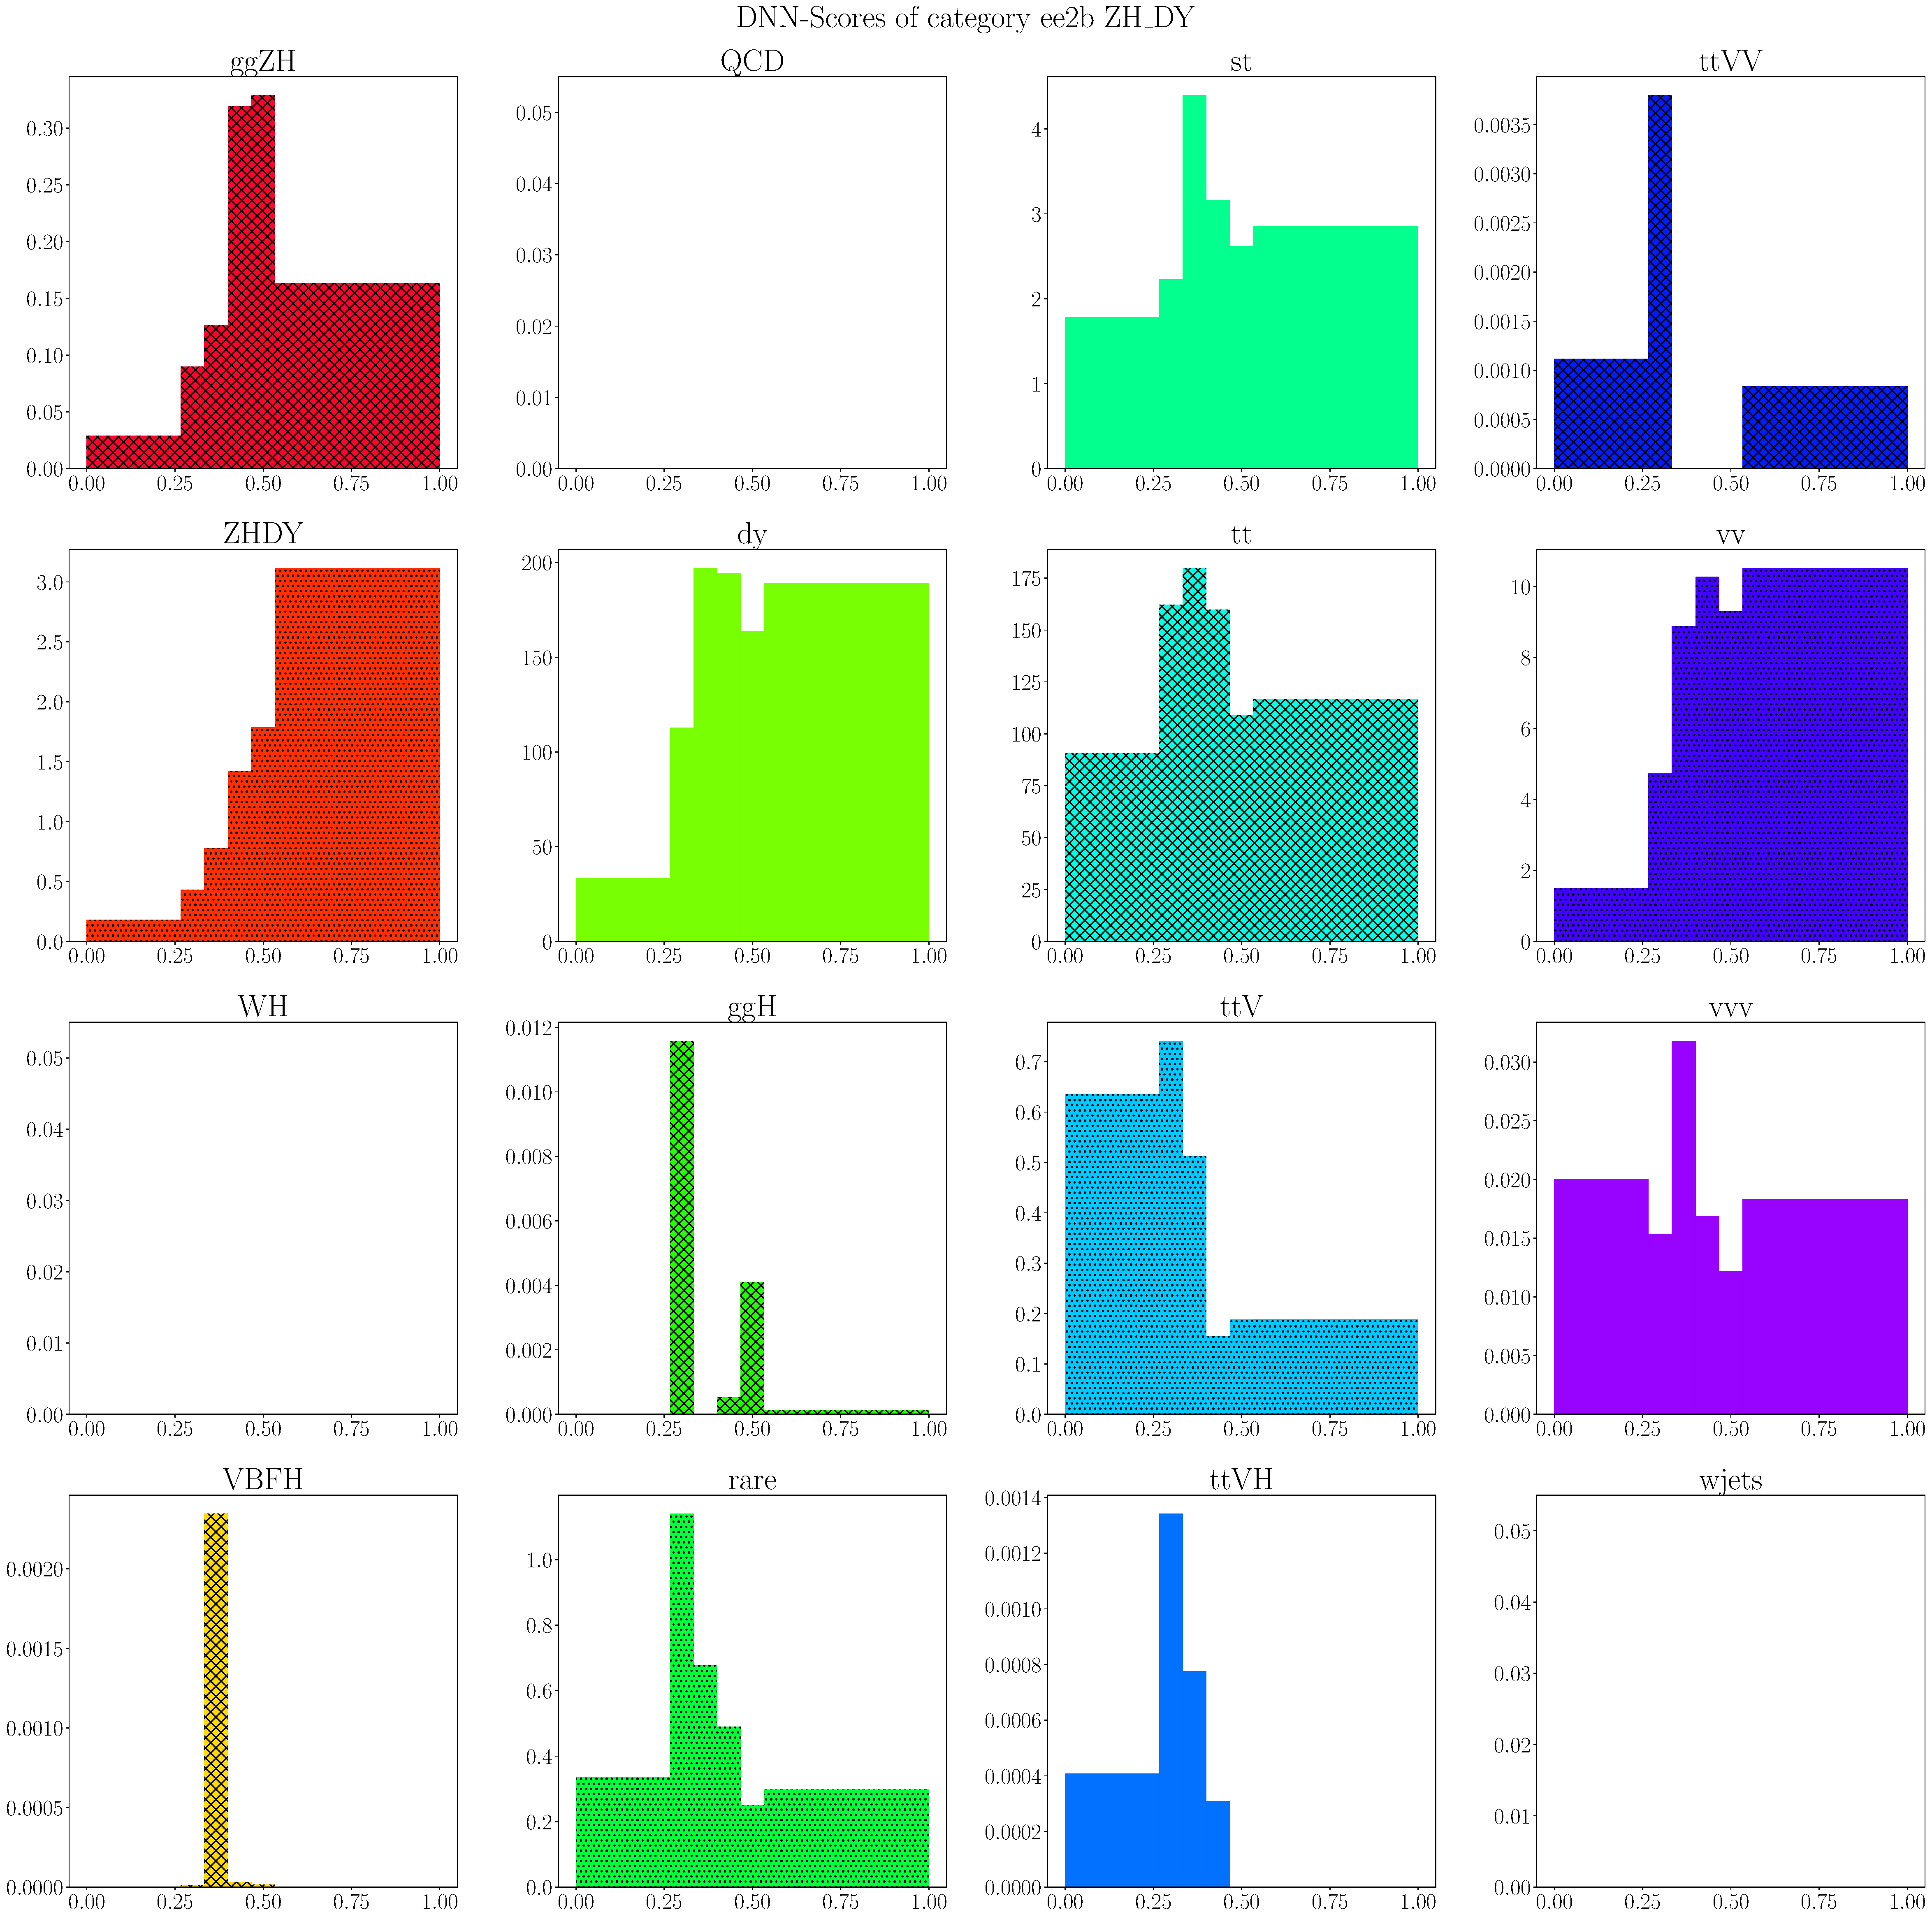
\includegraphics[width=\linewidth]{figures/analysis/ee_2b_dnn_node_ZH_DY.pdf}
	\caption{The DNN score distribution for the categorised final state objects for the \texttt{ZH\_DY} subcategory. Note the the different norming of the y axis and the high share of $t\bar{t}$, \texttt{dy} and \texttt{ZH\_DY} processes. Due to the effective categorization none of the \texttt{WH}, \texttt{QCD} and \texttt{wjets} events landed in this category. This is one of the total 52 subcategories.}
	\label{fig:ZH_DY_sub}
\end{figure}

Unfortunately, no single process can be seen in a measured dataset. What is possible though, is to fit the data to the distribution of the DNN scores of every category. A such histogram for a single category is shown in fig. \ref{fig:ee_dnn_score}; for all four categories covered by this study, the resulting histogram in shown in fig. \ref{fig:conditions}. In case of a measured dataset, only the resulting bin heights would be visible on which an analytical likelihood fit can be performed extracting the contribution of each signal process from the bins.

\begin{figure}[h!]
	\centering
	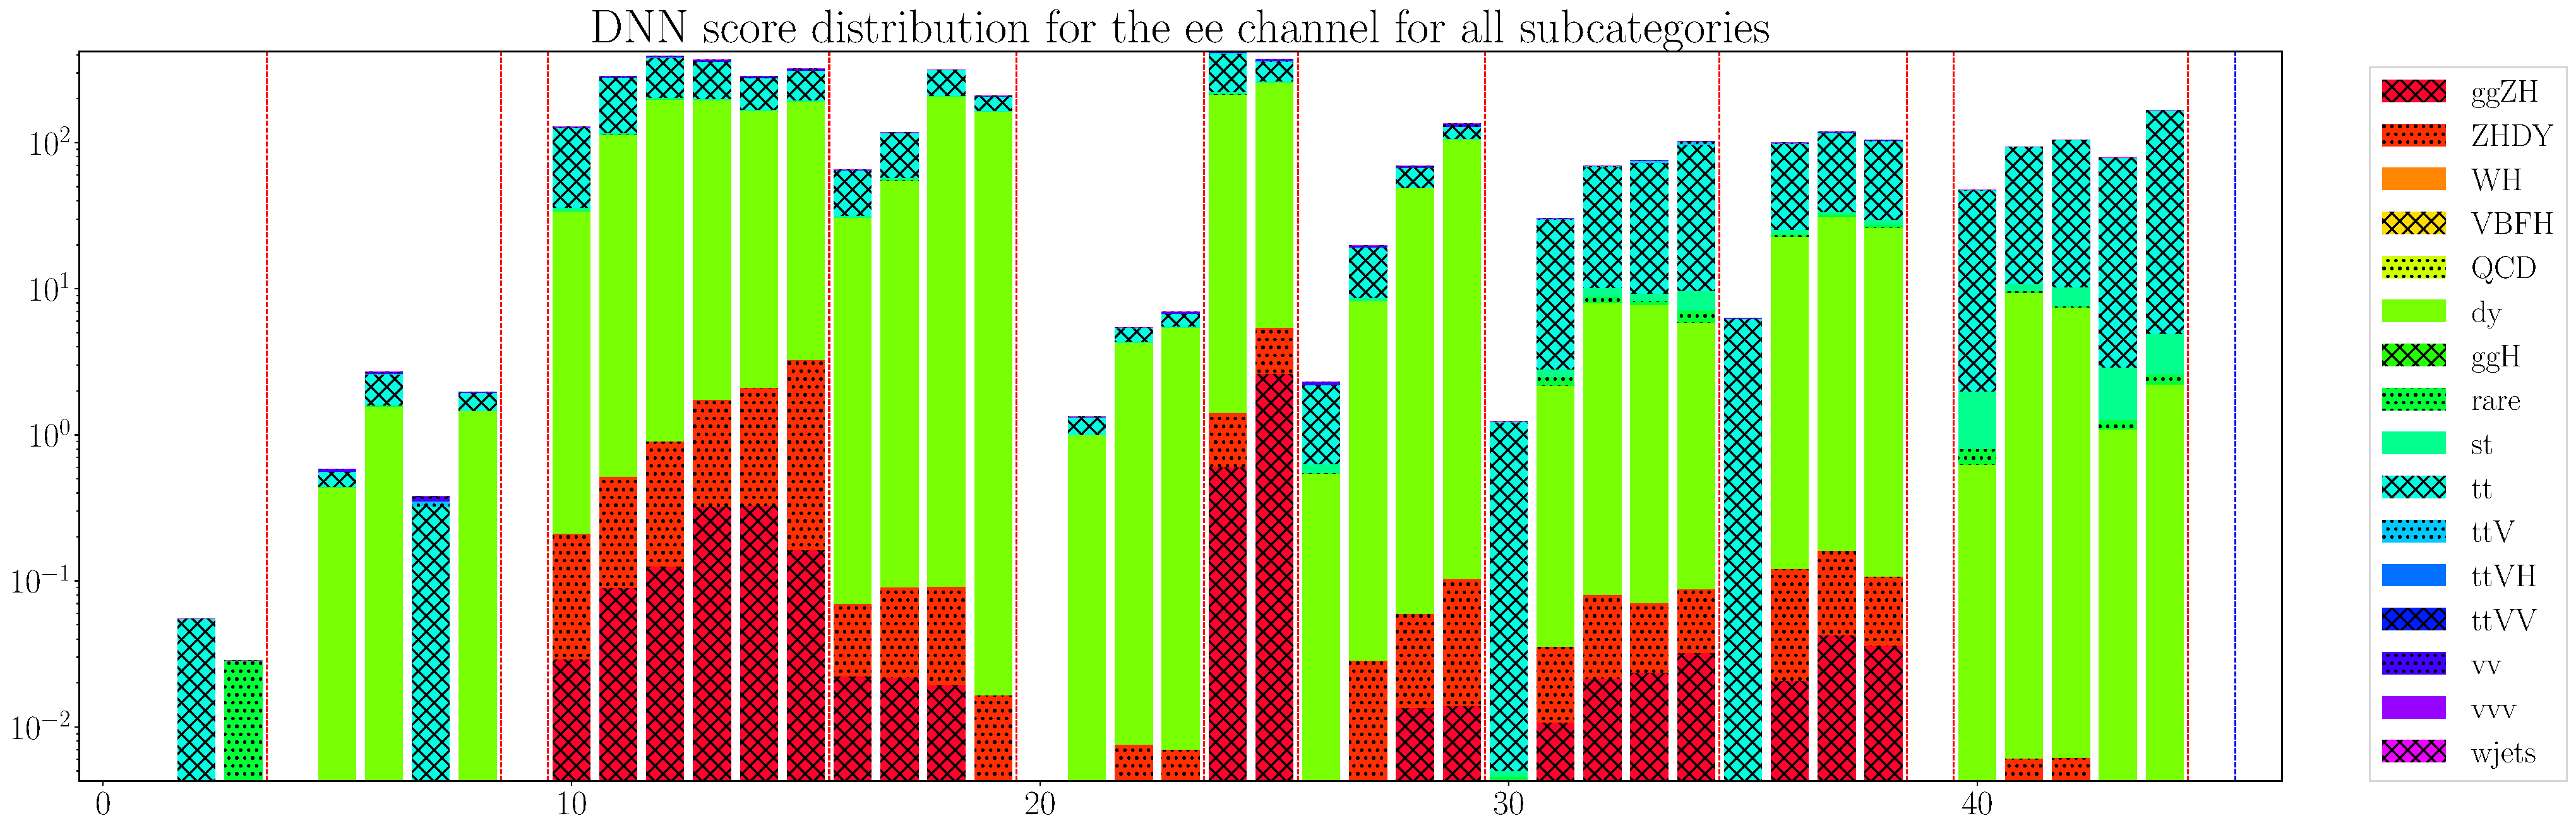
\includegraphics[width=\linewidth]{figures/analysis/cond1.pdf}
	\caption{The DNN score histogram distribution for the $ee$ category and each 13 subcategory (separated in red). On the x-axis, only the bin index is shown. The fourth subcategory from the left corresponds to the above-mentioned \texttt{ZH\_DY} subcategory. This is one of the four categories.}
	\label{fig:ee_dnn_score}
\end{figure}

\begin{figure}[h!]
	\centering
	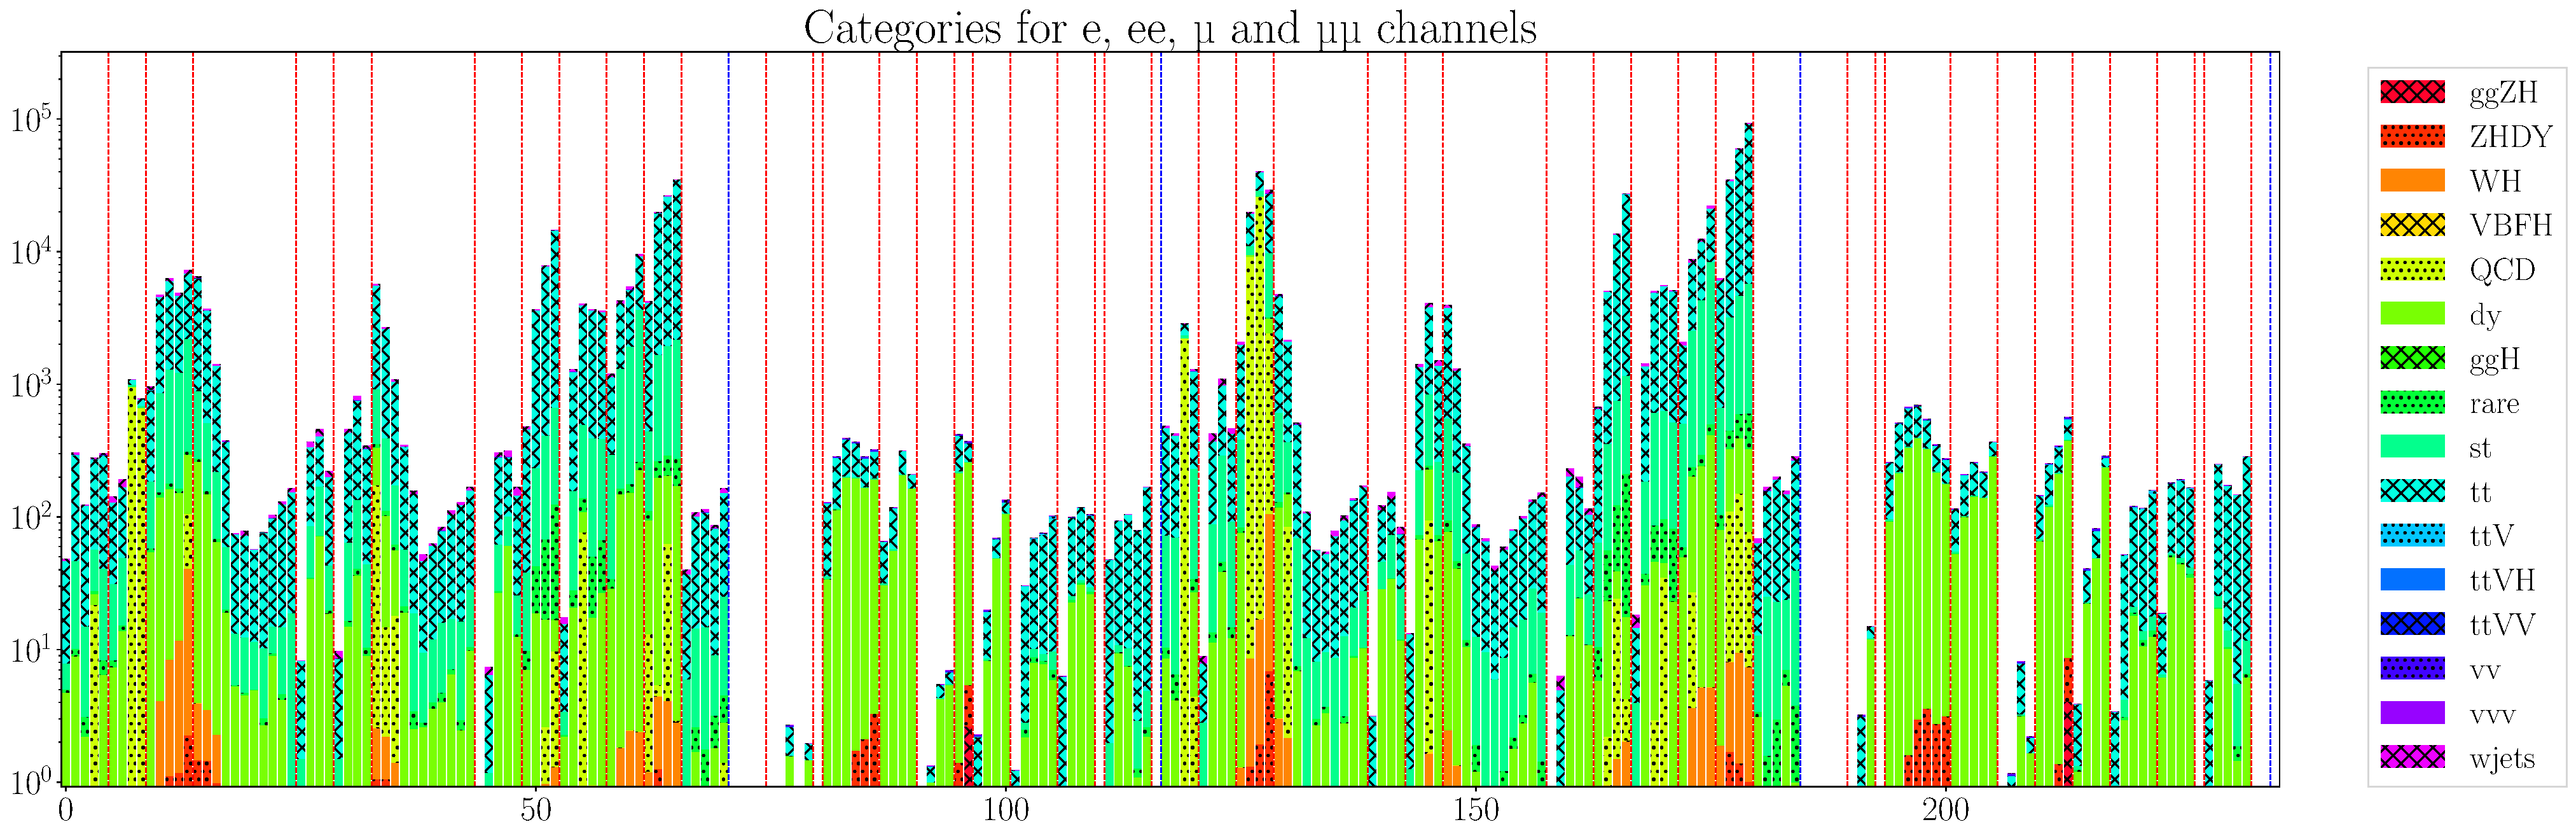
\includegraphics[width=1.1\linewidth]{figures/analysis/cond4_notOrdered.pdf}
	\caption{The distribution of the DNN scores for each subcategory (separated in red) in the semi- and dileptonic categories in consideration (separated in blue). Note the high share of Drell-Yan, $t\bar{t}$ and QCD background events in each bin and the absence of $WH$ events in the dileptonic bins. The $ee$ category is the second one from the left.}
	\label{fig:conditions}
\end{figure}

\Subsection{Likelihood Fits}

Using these histograms, the maximum likelihood fits can be performed to obtain the signal strength parameters. For that, the likelihood function for a signal+background hypothesis defined as

\begin{equation*}
	\mathcal{L}(N | \left\{\mu_i\right\} , \left\{\theta_i\right\}) = \prod\limits_i \frac{(\mu_is_i(\theta)+b_i(\theta))^N}{N!}e^{-\mu_is_i(\theta) + b_i(\theta)} \prod\limits_j p(\tilde{\theta}_j | \theta_j)
\end{equation*}

with Poisson-distributed binwise signal and background contributions $s_i$ and $b_i$ depending on the uncertainty-modelling nuisance parameter $\theta$ following the probability distribution $p(\tilde{\theta} | \theta)$ is fitted to the histogram. Note that this fit assumes only changes in the background processes within the uncertainties, but not in their proportion. In other words, there is a single signal strength modifier parameter for each signal process exclusively.

In this thesis, these signal strength modifier parameters will inferred using a conditional invertible neural network and will be compared to their maximum likelihood counterpart.